\documentclass[dvipdfmx]{beamer}
\usepackage{bxdpx-beamer}% dvipdfmxなので必要
\usepackage{pxjahyper}% 日本語で'しおり'したい
%\usepackage{etex}
%\usetheme{Warsaw}
\usetheme{Malmoe}
%\usetheme{AnnArbor}
%\usetheme{Hannover}
%\usetheme{Bergen}
%\usetheme{Berlin}
%\usetheme{Singapore}
%\usetheme{Montpellier}
%\usetheme{Pittsburgh}
\usepackage{graphicx}
\usepackage{latexsym,amssymb}
%\usepackage{epsbox}
%\usepackage{multirow}
\usepackage{fancybox}
\usepackage{fancyvrb}
%\usepackage{listings}
\usepackage{tabularx}
\usepackage{tikz}
%\usepackage{pstricks,pst-node,pst-tree}
%\usepackage{multimedia}
%\usepackage{pstricks,pst-node,pst-tree}
%\usepackage{pst-all}
%\include{prooftree}
%\lstloadlanguages{pascal}
\renewcommand{\kanjifamilydefault}{\gtdefault}
\renewcommand{\familydefault}{\sfdefault}
\graphicspath{{fig251104/}}
%\include{cmacros}

\newcommand{\greentext}[1]{{\color[rgb]{0,0.5,0}{#1}}}
\newcommand{\redtext}[1]{{\color[rgb]{0.8,0,0}{#1}}}
\newcommand{\bluetext}[1]{{\color[rgb]{0,0,0.8}{#1}}}

\newcommand{\tuple}[1]{\langle{#1}\rangle}

\newcommand{\First}{\mathsf{First}_1}
\newcommand{\Follow}{\mathsf{Follow}_1}

%%pdt simulation

\newcommand{\pdtline}[6]{%
    \uncover<#6->{
        \node at (${#5}*(0,-.3)+(0,.3)$) {$\vdash$};%
        \node at (${#5}*(0,-.3)+(1.5,.3)$) {\parbox{12em}{(#1,}};%
        \node at (${#5}*(0,-.3)+(4.5,.3)$) {\parbox{10em}{#2,}};%
        \node at (${#5}*(0,-.3)+(5.7,.3)$) {\parbox{10em}{#3)}};%
        \node at (${#5}*(0,-.3)+(8,.3)$) {\parbox{20em}{#4}};%
    }
}

\newcommand{\initpdtline}[6]{%
    \uncover<#6->{
        \node at (${#5}*(0,-.3)+(1.5,.3)$) {\parbox{12em}{(#1,}};%
        \node at (${#5}*(0,-.3)+(4.5,.3)$) {\parbox{10em}{#2,}};%
        \node at (${#5}*(0,-.3)+(5.7,.3)$) {\parbox{10em}{#3)}};%
        \node at (${#5}*(0,-.3)+(8,.3)$) {\parbox{20em}{#4}};%
    }
}

\newtheorem{Def}{定義}
\newtheorem{Lem}{補題}
\newtheorem{Thm}{定理}
\newtheorem{Prop}{命題}

\definecolor{lightlightgrey}{rgb}{0.95,0.95,0.95}

\newcommand{\ttpl}{\texttt{+}}
\newcommand{\ttsb}{\texttt{-}}
\newcommand{\ttmu}{\texttt{*}}
\newcommand{\ttdv}{\texttt{/}}
\newcommand{\tteq}{\texttt{=}}




%\newcommand{\greentext}[1]{{\color[rgb]{0,0.5,0}{#1}}}
%\newcommand{\redtext}[1]{{\color[rgb]{0.8,0,0}{#1}}}

\newcommand{\lecturedate}{2025/11/4}

\cornersize{0.25}

\setbeamertemplate{frametitle}[default][center]
\setbeamertemplate{footline}{\hfill
コンパイラ\quad\lecturedate
\hfill\insertframenumber/\inserttotalframenumber\hspace*{1zw}}
\newcounter{coffee}
\setbeamercovered{transparent=10}
\title{コンパイラ(10)}
\date{\lecturedate}
\begin{document}

\frame{\titlepage}

\section{構文主導型変換}

\subsection{中間コード生成ルーチン}

\begin{frame}
 \frametitle{PDTを用いた構文主導型変換}
 \greentext{コード生成を行うタイミング=還元操作}
 \begin{center}
  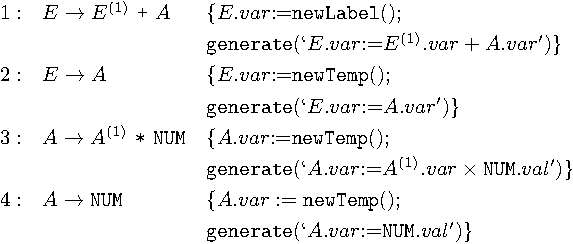
\includegraphics[scale=0.6]{bup-SDD-r1-crop.pdf}
 \end{center}
 \begin{center}
  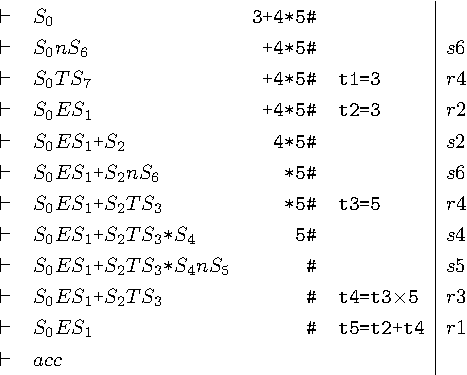
\includegraphics[scale=0.5]{IR-gen-crop.pdf}
 \end{center}
\end{frame}

\begin{frame}
 \frametitle{変換例}
 \[
  \begin{array}{ll}
   E_1\rightarrow a\ast b & \{\%0=a\ast b\}\\
   E_2\rightarrow -d & \{\%1=-d\}\\
   E_3\rightarrow c\ast E_2 & \{\%2=c\ast\%1\}\\
   E_4\rightarrow E_1+E_2 & \{\%3=\%0+\$2\}\\
   S\rightarrow x\texttt{:=}E_3 & \{x=\%3\}
  \end{array}
 \]

\begin{tikzpicture}
 \node (X0) at (0,0) {$x$};
 \node (T1) at (0.75,0) {$:=$};
 \node (T2) at (1.5,0) {$a$};
 \node (T3) at (2,0) {$\ast$};
 \node (T4) at (2.5,0) {$b$};
 \node (T5) at (3,0) {$+$};
 \node (T6) at (3.5,0) {$c$};
 \node (T7) at (4,0) {$\ast$};
 \node (T8) at (4.5,0) {$-$};
 \node (T9) at (5,0) {$d$};
 \uncover<2->{\node (T10) at (2,1) {$E_1$};}
 \uncover<3->{\node (T11) at (4.75,1) {$E_2$};}
 \uncover<4->{\node (T12) at (3.5,2) {$E_3$};}
 \uncover<5->{\node (T13) at (3,3) {$E_4$};}
 \uncover<6->{\node (T14) at (2,4) {$S$};}

 \uncover<2->{\path[-] (T2) edge (T10) (T3) edge (T10) (T4) edge (T10);}
 \uncover<3->{\path[-] (T8) edge (T11) (T9) edge (T11);}
 \uncover<4->{\path[-] (T6) edge (T12) (T7) edge (T12) (T11) edge (T12);}
 \uncover<5->{\path[-] (T10) edge (T13) (T5) edge (T13) (T12) edge (T13);}
 \uncover<6->{\path[-] (X0) edge (T14) (T1) edge (T14) (T13) edge (T14);}

 \only<2->{\node (N10) at (2.5,1) {\redtext{$\%0$}};}
 \only<3->{\node (N11) at (5.25,1) {\redtext{$\%1$}};}
 \only<4->{\node (N12) at (4,2) {\redtext{$\%2$}};}
 \only<5->{\node (N13) at (3.5,3) {\redtext{$\%3$}};}
 \only<6->{\node (N14) at (2.5,4) {\redtext{$\%4$}};}
 
 \only<2->{\node[anchor=west] at (6,3.5) {$\%0=a\ast b$};}
 \only<3->{\node[anchor=west] at (6,3) {$\%1=-d$};}
 \only<4->{\node[anchor=west] at (6,2.5) {$\%2=c\ast\% 1$};}
 \only<5->{\node[anchor=west] at (6,2) {$\%3=\$ 0+\% 2$};}
 \only<6->{\node[anchor=west] at (6,1.5) {$x=\%3$};}
\end{tikzpicture}
\end{frame}

\begin{frame}
 \frametitle{条件分岐に対する構文主導型変換}

 %\greentext{LR項の状態に対してコード生成}
 
\greentext{分岐条件の評価の後に分岐命令を生成する必要がある．}

\vfill

 \begin{tabular}{cc}
  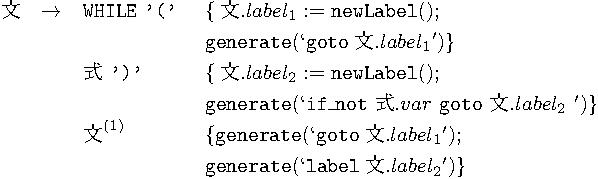
\includegraphics[width=.7\textwidth]{whileTrans-r1-crop.pdf} &
  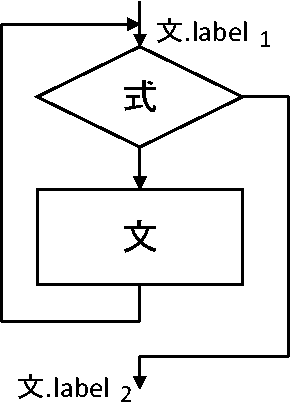
\includegraphics[width=.2\textwidth]{whileFlow-crop.pdf}
 \end{tabular}

%  \begin{trivlist}
%   \item  $\mathsf{newLabel}(\&\mbox{文}.label_1)$:\\
% 	 新たなラベルを生成して,$\mbox{文}.label_1$の値を更新する.
%   \item $\mathsf{generate}(s1,s2,\ldots)$:\\
% 	$s_1,s_2,\ldots$ の命令部分を結合して命令を生成する.
%   \item $\mbox{式}.var$:\\
% 	式のコード生成の結果が格納される変数
%  \end{trivlist}
 
\end{frame}

\begin{frame}[fragile]
 \frametitle{while文の中間コード生成例}
\begin{center}
 \begin{Verbatim}
  while(x<20) {
    r=r+x;
    x=x+1
  }
 \end{Verbatim}
\end{center}
  \begin{tabular}{cc}
   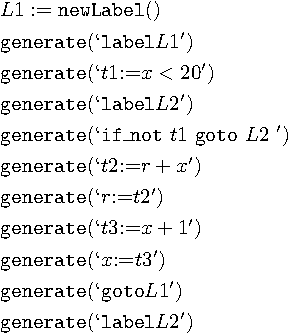
\includegraphics[width=.3\textwidth]{whileCodeExample-r1-crop.pdf}
   &
   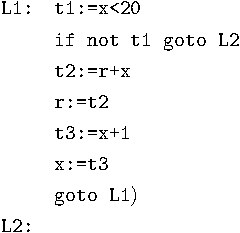
\includegraphics[width=.3\textwidth]{whileCode-crop.pdf}
   \\
  \end{tabular}
\end{frame}

\begin{frame}
 \frametitle{上昇型構文解析におけるコード生成}

\begin{trivlist}
\item IF文
{\small
\[\begin{array}{rcll}
  I & \rightarrow & \texttt{if}\ \texttt{(}\ E\ \texttt{)}
  & \{S.label1\mbox{:=\makenewlabel};\\
  & & & \genifnot{E.var}{S.label1}\}\\
  S'& \rightarrow\  & I S^{(1)} & \{S'.label:=\makenewlabel;\\
  & & & \gengoto{S'.label};\\
  & & & \genlabel{I.label}\}\\
  S & \rightarrow & S'\ \texttt{else}\ S^{(2)} & \{\genlabel{S'.label}\}\\
 \end{array}\]}
\item WHILE文
{\small
 \[\begin{array}{rcll}
  I & \rightarrow & \texttt{while}\ \texttt{(} & \{I.label\mbox{:=}\makenewlabel;\\
    & & & \genlabel{I.label}\}\\
  S' & \rightarrow & E\ \texttt{)} & \{S'.label:=\makenewlabel;\\
    & & & \genifnot{E.var}{S'.label}\}\\
  S & \rightarrow & IS'S^{(1)} & \{\gengoto{I.label};\\
    & & & \genlabel{S'.label}\}
 \end{array}\]}
\end{trivlist}
\end{frame}

\begin{frame}
 \frametitle{下降型構文主導型変換}
 構文図式に従ってコードを生成する。

 \greentext{丸}の部分でコードを生成する

 \begin{center}
  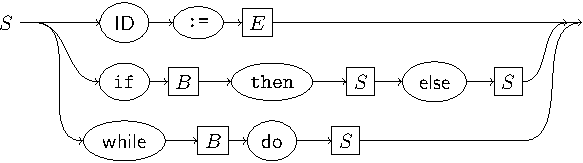
\includegraphics[scale=.8]{synDiag-S-crop.pdf}
 \end{center}
\end{frame}

\begin{frame}
  \begin{center}
    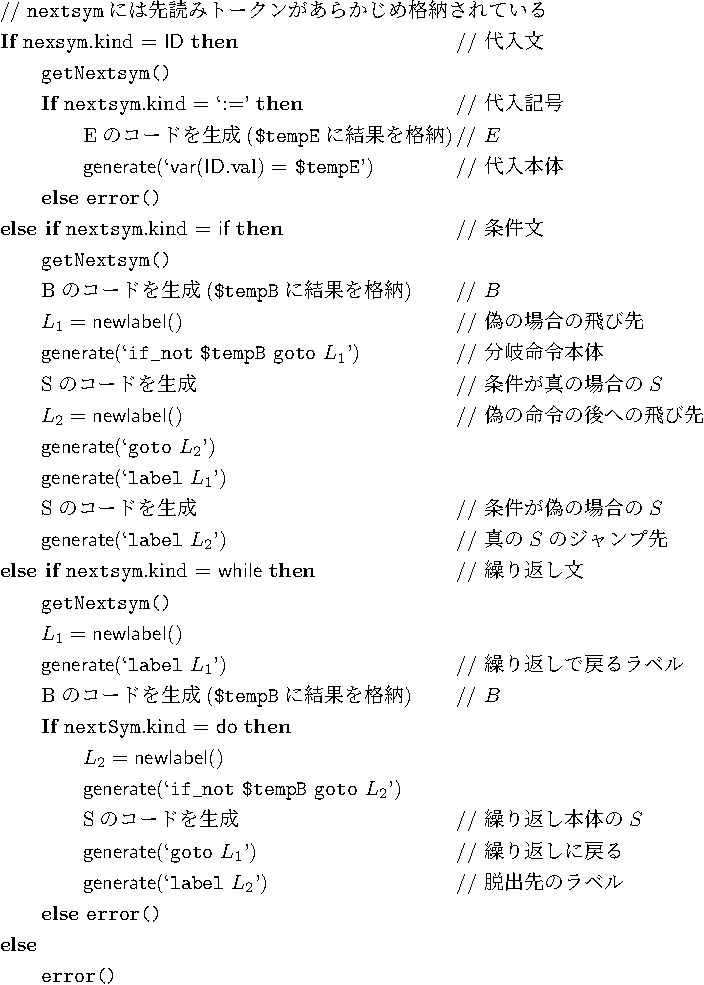
\includegraphics[scale=.5]{recDescent-gen-crop.pdf}
  \end{center}
\end{frame}

\end{document}
